%synthese
Les botnets font maintenant partie d'une économie souterraine sous forme de services payants.
Le harcèlement, le vol, les attaques par déni de service, etc figurent comme des produits de vente accessibles, moyennant finances, pour n'importe quel criminel.
\newline D'après l'ENISA\footnote{European Union Agency for Cybersecurity, anciennement European Network and Information Security Agency} les prix varient suivant la fiabilité, la durée et le type de service requis.
Par exemple une heure de DDoS est disponible pour 38\$.
Les différentes architectures permettent de mieux comprendre l'organisation du botnet et l'importance du C\&C.
\vspace{5mm}
\newline Les notions de veille technologique et de partage d'informations sur la menace sont essentielles du fait de l'implication du botnet dans les réseaux publiques et privés.
\newline Dans le cadre du renseignement lié aux menaces, les constructeurs de smartphone fournissent les informations (recherches,cible des attaques, menaces associés aux mobiles, vulnérabilités des objets IoT) issues de leurs Threat Intelligence Center\footnote{Centre de renseignements liés aux menaces cyber}.
%ouverture
\vspace{5mm}
\newline Selon Nokia (\href{https://www.nokia.com/about-us/news/releases/2018/12/04/nokias-threat-intelligence-report-2019-warns-on-the-fast-growing-and-evolving-threat-of-malicious-software-targeting-internet-of-things-iot-devices/}{Nokia's Threat Intelligence Report}, l'activité des botnet sur l'IoT représente 78\% des événements de détection de malware en 2018.
\newline La menace omniprésente de ces objets connectés (santé, domotique, médias, électroménager,...) n'est aujourd'hui pas assez prise en considération par notre société de consommation.
Le manque de sécurité accrue de ces appareils faits apparaître ces objets connectés comme des acteurs potentiels constituant le réseau d'un botnet.
\newline L'arrivée prochaine de la 5G\footnote{prévisions en moyenne 100Mbit/S en download et 50 Mbit/s en upload} sera, dans ce domaine, un vecteur majeur pour la diffusion de l'infection du malware et le nombre d'attaques associés au botnet (exemple attaques DDoS).
\begin{figure}[h!]
\begin{center}
	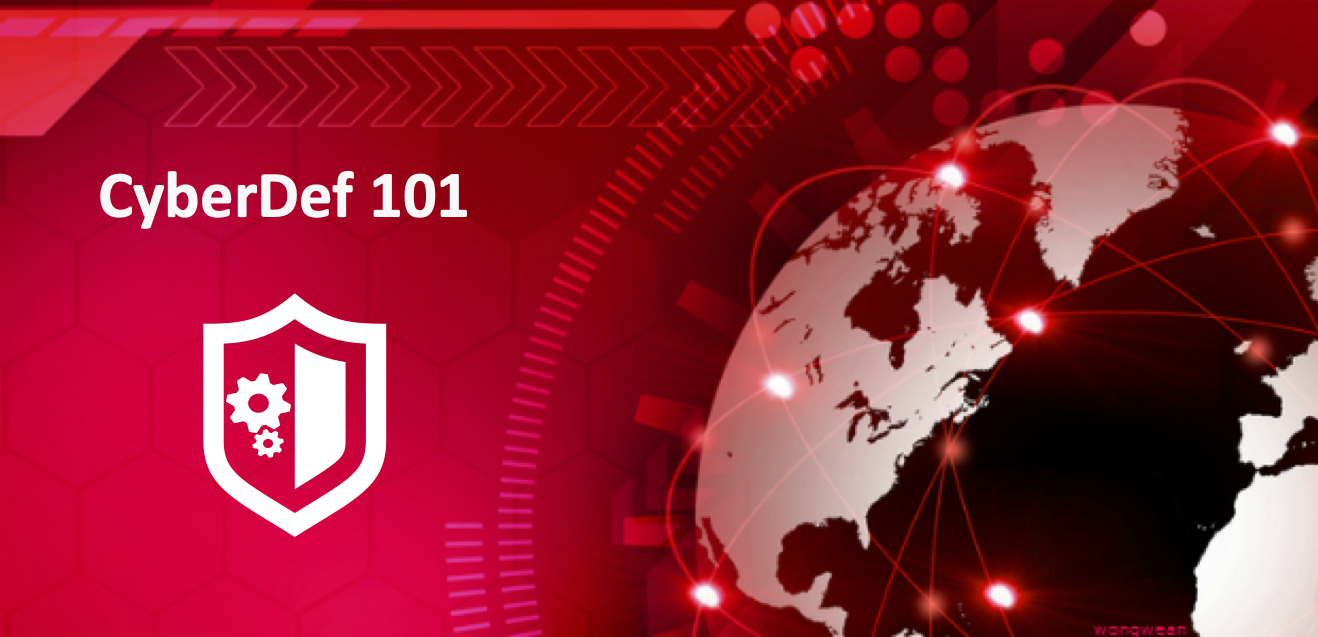
\includegraphics[width =0.6\textwidth, keepaspectratio]{coverback}
	\caption{Figure 1}\label{mon image}
	\end{center}
\end{figure}